\documentclass[a4paper, 12pt]{article}
\usepackage{graphicx}
\usepackage[utf8]{inputenc}
\usepackage{multirow}
%\usepackage{times}
\usepackage{listings}
\usepackage{supertabular}
\usepackage{cite}
\usepackage{amsthm}
\usepackage{tikz}
\newcommand*\circled[1]{\tikz[baseline=(char.base)]{
            \node[shape=circle,draw,inner sep=2pt] (char) {#1};}}
\newcommand{\todo}[1]{\ensuremath{^{\textrm{\tiny{TODO}\normalsize}}}\footnote{\textbf{TODO:}~#1}}

\newcommand{\jcode}[1]{\textnormal{\texttt{#1}}}
\newcommand{\pcode}[1]{\textnormal{\texttt{#1}}}
\newcommand{\pmodule}[1]{\textnormal{\texttt{#1}}}
\newcommand{\rdfterm}[1]{\textnormal{\textsf{#1}}}

\include{helpers}
\usepackage[pdftex,linktocpage]{hyperref}
\hyperbaseurl{https://github.com/}

\begin{document}
\title{Prefetching SPARQL query cacher}
\author{Kjetil Kjernsmo}
%\institute{Department of Informatics,
%Postboks 1080 Blindern,
%0316 Oslo, Norway}

%\email{kjekje@ifi.uio.no}

\maketitle

\section{Introduction}

This chapter describes an effort to create a proxy that can cache the
results of not only SPARQL queries, but also the results of individual
triple patterns. It will asynchronously analyse executed queries, and
may prefetch the results of certain triple patterns into the cache.

The system is in the convergence of the directions described in this
dissertation: It should relieve the remote endpoint of some of the
burden to evaluated the query and it should add to the robustness of the
open Web SPARQL infrastructure. It uses hypermedia to answer individual
triple patterns, based on Triple Pattern Fragments  \cite{ldf1}. The
system can only answer triple patterns, but other than that, supports
SPARQL 1.1 in its entirety. This was made possible to develop quickly
by the efforts put into the query planning in the Attean framework
described in Section~\ref{sec:conpush}. Caching based on RFC7234
\cite{rfc7234} was shown to be of possible use in the survey I
conducted. Finally, it was planned to be evaluated using
Design of Experiments.

Unfortunately, the system has as of this writing insufficient
performance for an evaluation to be meaningful. Nevertheless, it
points out some interesting lessons with varying degrees of
certainty. This chapter will detail the system, show its design and
features and discuss its failures.

Figure~\ref{fig:messaging} illustrates where caches may be in the
Internet infrastructure, as well as HTTP requests and responses in a
typical deployment scenario of the system.

\begin{figure}
\begin{center}
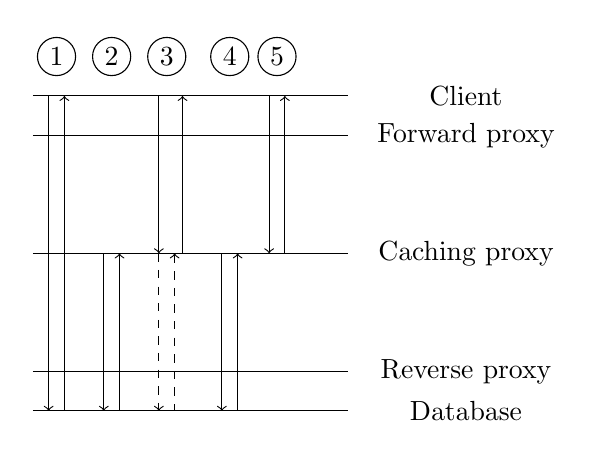
\begin{tikzpicture}
\draw (0,0) --(4,0);
\node at (5.5,0) { Database };
\draw (0,0.5) --(4,0.5);
\node at (5.5,0.5) { Reverse proxy };
\draw (0,2) --(4,2);
\node at (5.5,2) { Caching proxy };
\draw (0,3.5) --(4,3.5);
\node at (5.5,3.5) { Forward proxy };
\draw (0,4) --(4,4);
\node at (5.5,4) { Client };

\draw [->] (0.2,4) --(0.2,0);
\draw [<-] (0.4,4) --(0.4,0);
\node at (0.3,4.5) {\circled{1}};
\draw [->] (0.9,2) --(0.9,0);
\draw [<-] (1.1,2) --(1.1,0);
\node at (1.0,4.5) {\circled{2}};
\draw [->] (1.6,4) --(1.6,2);
\draw [dashed, ->] (1.6,2) --(1.6,0);
\draw [dashed, <-] (1.8,2) --(1.8,0);
\draw [->] (1.9,2) --(1.9,4);
\node at (1.7,4.5) {\circled{3}};
\draw [->] (2.4,2) --(2.4,0);
\draw [<-] (2.6,2) --(2.6,0);
\node at (2.5,4.5) {\circled{4}};
\draw [->] (3,4) --(3,2);
\draw [->] (3.2,2) --(3.2,4);
\node at (3.1,4.5) {\circled{5}};
\end{tikzpicture}
\caption{The possible positions of a cache. A cache may reside at both
  the server side (as a database cache) or client side, or any of the
  intermediate proxies. The arrows illustrate requests (when pointing
  down) and responses (when pointing up) in a deployment scenario for
  when a the query cache considered in this paper is deployed on a
  caching proxy in the Internet infrastructure, see the text for
  details.}\label{fig:messaging}
\end{center}
\end{figure}

The system is based on HTTP, which implies a client-server
architecture. In this architecture, a cache may be present at
conceptually five different levels. First, the client may have its own
cache, which caches only responses made by the client itself. The next
level is known as a forward proxy. They aren't currently very common,
but have in the past often been institutional proxies, or proxies
employed by Internet Service Providers for caching responses that may
be common to many of their users. The next level, generically referred
to as a caching proxy, may be in the Internet
infrastructure. Currently, the most common form of this type of proxy
is known as a Content Delivery Network (CDN). It is very common to
have a reverse proxy near the server. They are often known as a ``Web
Accelerator''. Usually, they will communicate with the server with
HTTP, but it is conceivable that it may use a different protocol, and
may employ detailed knowledge of the hosted data to optimise cache
operations. Finally, the database, in this context a SPARQL Endpoint,
may use conventional database caching techniques. The database cache
and reverse proxy is typically controlled by the data provider.

The present system may be deployed at any of these levels. However,
since the database and the reverse proxy in front of it may have
detailed knowledge of the data, e.g. a complete data profile with
statistics to optimise join order, these levels have much in common
with a conventional database cache, which is extensively discussed in
the literature.

My interest is the case where the caching proxy has no further
knowledge of the data than what is exposed through the SPARQL Endpoint
or hypermedia metadata. In practice, there is very little
information. If the cache is to be shared, then it would typically
reside on the forward proxy, or in a CDN. 

Figure~\ref{fig:messaging} illustrates the case where HTTP messages
are being passed, where the cache is assumed to reside on a
intermediate caching proxy in the Internet, i.e. a CDN. The figure may
be viewed as having time on the $x$-axis, with the arrows pointing
down being requests and the arrows point up being responses. In this
example, the client first makes a request (request \circled{1}), which
is passed through the proxy because it has not yet cached any
responses. The response (response \circled{1}) is then also
transmitted directly from the SPARQL Endpoint at the database back to
the client. The entire response may be cached at the proxy in case it
can be reused in its entirety. However, the main point is that the
request will be analysed by the proxy in parallel to being sent to the
server, and another request \circled{2} for a triple pattern fragment
that the analyser thinks will enable the proxy to assist the server
the best for future requests, is sent. This analysis is discussed in
\todo{ref}. The response \circled{2} is not sent back to the client,
but will enter the cache. Lets say that the analyser was successful
and that the cache can be used to answer request \circled{3}. In that
case, the proxy will send a rewritten query for the rest of the data
it needs to answer the query to the origin server, indicated by the
dashed arrows. This may be a SPARQL query, a TPF request or a
combination thereof, depending on what the planner finds least
expensive. The proxy will then evaluate the entire query and send the
final result back as response \circled{3}. In addition, the analyser
may have identified another Triple Pattern Fragment that it takes as
likely useful for future requests, and sends a request and caches the
response \circled{4}. At some point, it may be able to answer the
entire query using only cached results, as illustrated by request and
response \circled{5}.

\section{Implementation}\label{sec:impl}

The implementation consists of several modules that have been
published to the Comprehensive Perl Archive Network as Free Software,
and most of which have become a part the Free Software ecosystem. To
install the system on the top of a Debian system with only essential
packages requires 146 Debian packages. Running the test suite requires
even more. As such, it builds on the code of hundreds of authors, too
long to enumerate. I shall constrain myself to list the modules that
have code that has been motivated from this study. Modules that have
other primary authors than myself have been started prior to this
present project, but may have substantial contributions from this
project. The Attean framework was started as part of the effort in
Section~\ref{sec:conpush}, but even though it has been developed
further with the requirements that arose from this project and has
contributions from me, the vast majority of the code has been written
my Gregory Todd Williams. The main work in this project has gone into
the module \pmodule{AtteanX::Query::Cache}, where I have authored the vast
majority of the code. The relative difference in authorship can be
further examined by checking the linked Github repositories, or by
using git2prov\footnote{see \url{http://git2prov.org/}} to create RDF
data of the commit history. Table~\ref{tab:modules} shows the modules
that have been influenced or written as part of this project.

\begin{table}
\caption{The modules that enable the query cache}\label{tab:modules}
\begin{tabular}{ | l | p{3cm} | l |}
  \hline
  Module & Authors & Github URL \\ \hline

  \pmodule{AtteanX::Query::Cache} & Kjetil Kjernsmo, Gregory Todd Williams &
  \url{kjetilk/p5-atteanx-query-cache} \\ % 0.001_04

  \pmodule{AtteanX::Store::SPARQL} & Kjetil Kjernsmo &
  \url{kjetilk/p5-atteanx-store-sparql} \\ % 0.008
  
  \pmodule{AtteanX::Store::LDF} & Kjetil Kjernsmo, Patrick Hochstenbach &
  \url{phochste/AtteanX-Store-LDF} \\ % 0.02

  \pmodule{LWP::UserAgent::CHICaching} & Kjetil Kjernsmo &
  \url{kjetilk/p5-lwp-useragent-chicaching} \\ % 0.04
  
  \pmodule{Attean} & Gregory Todd Williams, Kjetil Kjernsmo &
  \url{kasei/attean} \\ % 0.015

  \pmodule{AtteanX::Endpoint} & Gregory Todd Williams &
  \url{kasei/atteanx-endpoint} \\ % 0.001

  \pmodule{RDF::LDF} &  Patrick Hochstenbach, Gregory Todd Williams, Jakob Voß,
  Kjetil Kjernsmo & \url{phochste/RDF-LDF} \\ % 0.17
  
  \hline
\end{tabular}
\end{table}

The system also depends on modules I have written that is not part of
the project: \pmodule{RDF::LinkedData}, \pmodule{RDF::Generator::Void}, \pmodule{Test::RDF},
\pmodule{URI::NamespaceMap} and \pmodule{RDF::NS::Curated}.

To further understand the roles of the different modules, note the
following: \pmodule{LWP::UserAgent::CHICaching} is a traits-based \cite{traits} implementation of the
majority of RFC7234. \pmodule{AtteanX::Endpoint} is an implementation of the
server side of SPARQL 1.1 Protocol. 

\subsection{The Attean framework}

The Attean framework was born from the experiences the PerlRDF
community gained with \pmodule{RDF::Trine}, the Perl counterpart to
the more well-known Jena framework, and the opportunities presented by
the introduction of traits \cite{traits}, or roles as they are known,
to the Perl world.

Traits are groups of methods that serve as a primitive unit of code
reuse. Traits are not constructed to objects themselves and do not
use inheritance for composition, instead a class is composed by a set of
traits and possibly the class' own methods, and then instantiated. A
trait can also require a set of methods, and as such, is similar to
interfaces, but since its focus is code reuse, it can also provide a
default implementation. 

The Attean framework packages commonly used classes when using
Semantic Web data, like RDF statements and terms, parsers,
serializers, triple/quad stores, iterators, but also features that are
relevant to query answering, like algebra, query planners and
plans. Additionally, it has an underlying extensive API consisting of
roles that can be composed to the above classes.

Perl is an interpreted language and is not known to run fast. Instead,
the focus is on developer efficiency. However, our motivation for
Attean, expressed in \cite{williamspushing}, was to enable the use
of faster implementations by using roles to simplify code reuse.

For this work, the usage of roles to simplify query planning is of
particular importance. While we do not exploit optimisations closer to
the database, we extend the query planner in several directions with
several separate add-on modules, with only generic functionality in
the core Attean framework.

We have found it convenient to use classical inheritance in
combination with traits-based composition, but only when the base
class provide only fundamental functionality that is very likely to be
common to all implementations. For an example of this, see
Section~\ref{sec:cacher}.

Also of importance are the APIs to compose stores. Stores in Attean
can be triplestores or quadstores, they can be mutable,
bulkupdateable, can enable the use of ETags or modification times for
conditional requests (as defined in RFC7232 \cite{rfc7234}, and makes
possible further extensions. Each of these primitives is represented
by a role that implements default functionality or simply requires
such functionality to be required. For instance, a quadstore is
required by \pmodule{Attean::API::QuadStore} to implement the
\pcode{get\_quads} method, which can take an RDF term as one or more
of the arguments and variables for the rest, and should return an
iterator over the quads that were matched. Based on an implementation
of the \pcode{get\_quads} method, the \pmodule{Attean::API::QuadStore}
role provides default implementations of methods \pcode{count\_quads},
\pcode{count\_quads\_estimate}, \pcode{get\_graphs} and
\pcode{size}. These methods may be overridden when composing a
class. Composing other roles will require further methods to be
implemented.\todo{Explain Model}

When a query is parsed, algebra objects are generated. Based on the
algebra tree, models (which may delegate the task to the store) may
generate plans for any algebra object of their choosing by
implementing the \pmodule{Attean::API::CostPlanner} role. This amounts
to implementing \pcode{plans\_for\_algebra} and
\pcode{cost\_for\_plan} methods. For a given algebra, Attean's query
planner will trust that the model's \pcode{plans\_for\_algebra} is
better than its own by default, a choice that was justified in
\cite{williamspushing}. Additionally, Attean has a simpler mechanism
for single triple or quad patterns: By default, triple or quad
patterns are evaluated by calling the store's \pcode{get\_triples} or
\pcode{get\_quads}, but this may be augmented by adding a wrapper
around an \pcode{access\_plans} method used by the query planner to
produce further plans.

Based on the algebra tree and plans generated by the models or the
default query planner, as well as the access plans, several
alternative plans will be generated, and their cost will be
estimated. How this happens in detail depends on how the planner is
composed. Attean comes with two roles that implement different
planners, \pmodule{Attean::API::SimpleCostPlanner} will compute all
possible plans and then estimate the cost of all plans, and finally
return the best 5. \pmodule{Attean::API::IDPJoinPlanner}, which
implements an Iterative Dynamic Programming planner
\cite{Kossmann:2000:IDP:352958.352982}, which prunes plans
aggressively based on their estimated cost in each iteration of query
plan generation. When a final plan tree has been found, the query may
be executed. 

That new plan types can be integrated into the planner with ease, and
that the planner itself can be changed with very little effort is a
key contribution of the Attean system, which I have taken advantage of
in this work. That this is made easy is to the credit of traits, as
will become clear as we study the details of the implementation in
Section~\ref{sec:cacher}.


\subsection{SPARQL protocol client}

The \pmodule{AtteanX::Store::SPARQL} module is a partial SPARQL
Protocol client that implements Attean APIs. The store implementation
itself composes the TripleStore API and implements methods to retrieve
the results of a single triple pattern and exact cardinality for a
given triple pattern, by using an aggregate query. In addition, it can
generate plans for Basic Graph Pattern algebra objects that have more
than one triple pattern. If that is the case, it will return an
instance of the class \pmodule{AtteanX::Plan::SPARQLBGP}, which is
also defined by the module. If it is not the case, the module also has
an implementation of the \pcode{access\_plan} method in a
\pmodule{AtteanX::Query::AccessPlan::SingleQuadBGP} role, that can be
composed by a query planner to provide a single triple pattern
\pmodule{AtteanX::Plan::SPARQLBGP} object. Finally, it also provides a
model implementation that composes the Model and CostPlanner
APIs. This contains a \pcode{cost\_for\_plan} implementation that will
provide a cost for \pmodule{AtteanX::Plan::SPARQLBGP} objects that are
proportional to the number of triple patterns in the plan, but
penalises plans that does not have triple patterns that are connected
through a variable (i.e. will cause a Cartesian join) with a factor
10. See Section~\ref{sec:costheuristics} for details on the cost
heuristics.

\subsection{Linked Data Fragment client}\label{sec:ldfclient}

The Linked Data Fragment client work was started prior to this project
by Patrick Hochstenbach, and consists of the client code for Triple
Pattern Fragments in \pmodule{RDF::LDF}. It also includes the Basic
Graph Pattern optimisation from \cite{verborgh2014querying}. Included with the client
code is an implementation of a triple store of the legacy
\pmodule{RDF::Trine} framework that predates Attean. He also started
an Attean store implementation \pmodule{AtteanX::Store::LDF} as a
separate module, but that module was subsequently adopted by me, and I
have written most of the functionality. It composes the TripleStore
and CostPlanner APIs and implements triple pattern queries and
cardinality estimates, both provided by the underlying client code as
they are a part of the core functionality of Triple Pattern Fragments,
as well as \pcode{cost\_for\_plan}.

It also supplies a plan class \pmodule{AtteanX::Plan::LDF::Triple}
used in the query planning. 

\subsection{The caching proxy}\label{sec:cacher}

The caching proxy consists of several components:

\begin{itemize}
\item Analysers, used to determine whether certain triple patterns
  should have their results prefetched and cached.
\item A prefetcher that performs the needed actions.
\item Two query planners, one that can use a local cache and a remote
  endpoint, and another that extends this to be able to use Triple
  Pattern Fragments as well, and corresponding models.
\item Two roles to generate plans for accessing cache and Triple
  Pattern Fragments and a corresponding plan class to enter results
  in the cache.
\item A custom User Agent for caching.
\item The actual caching proxy that accepts queries, runs the planner
  and returns the results.
\item Scripts to run the whole system.
\end{itemize}

\subsubsection{Analysis and prefetching}

Analysers and prefetchers run asynchronously with query
evaluation. This is achieved by an addition to the proxy that sends a
query to a persistent analyser script that subscribes to a channel on
a Redis\footnote{See \url{http://redis.io/}} data structure store. 

The analyser script can be configured to use any number of analysers.
Two such analysers have been implemented, for now constrained to
single triple patterns. One will count the predicates in consecutive
queries it sees, and publish triple patterns to another Redis channel
with the predicate if the count exceeds a certain configurable
limit. This is an attempt to capture and cache popular parts of
queries.

The second analyser will rerun the query planner on the incoming query
while simulating that the results of a certain triple pattern was in
the cache. If the cost reduction of the best plan is larger than a
configurable limit, it will publish that triple pattern to the same
Redis channel as above. 

Another persistent script is subscribed to this latter channel. If the
Model supports Linked Data Fragments, a retriever will then download
the results of the triple pattern and enter it into the cache, or use
a single triple pattern SPARQL query if not.

The cache itself is assumed to only cache triples where at least one
term is bound. I have used the Redis data structure store for the
cache as well. This choice is somewhat arbitrary, and has not proved
very successful. The cache will store the results as an array if two
RDF terms were bound in the triple pattern, or a hash if only one term
was bound. The strings put into the cache are serialized N-Triples
strings.

In addition to caching the prefetched results, the proxy may also
cache the serialized results of any full SPARQL query, and also enter
the results of any Linked Data Fragment retrieved when the query
planner evaluates a query into the above cache, using a trivial
extension to the plan class in Section~\ref{sec:ldfclient}.



\subsubsection{Query planner}

For example, the query planner that can use a local cache and a remote
endpoint, named \pmodule{AtteanX::QueryPlanner::Cache}, extends the
basic query planner of the Attean framework,
\pmodule{Attean::QueryPlanner}, but also composes the following roles:
\pmodule{Attean::API::NaiveJoinPlanner},
\pmodule{Attean::API::SimpleCostPlanner},
\pmodule{AtteanX::API::JoinRotatingPlanner},
\pmodule{AtteanX::Query::AccessPlan::SingleQuadBGP} and
\pmodule{AtteanX::Query::AccessPlan::Cache}. 



\bibliography{management,dataprofiles,federation,dynamicity,hypermedia,specs,webarch,practical,semweb,caching,critisism,data,philosophy,benchmarks,rfc,programming,egne}
\bibliographystyle{plain}

\end{document}
